\documentclass[tikz,convert, margin=3mm]{standalone}
\usetikzlibrary{arrows}
\usetikzlibrary{decorations.pathreplacing,decorations.markings}

\begin{document}
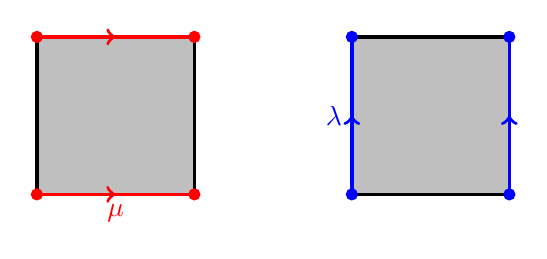
\begin{tikzpicture}
	\node at (0, 2) (a) {};
	\node at (2, 0) (c) {};
	\node at (2, 2) (d) {};
	\node at (0, 0) (o) {};
	\node[below, red] at (1, 0) (mu) {$\mu$};


	\node at (4, 2) (a) {};
	\node at (6, 0) (c) {};
	\node at (6, 2) (d) {};
	\node at (4, 0) (o) {};
	\node[left, blue] at (4, 1) (l) {$\lambda$};

	\filldraw[very thick, fill=black!25] (4,0) rectangle (6,2);
	\begin{scope}[very thick,decoration={
	    markings,
	    mark=at position 0.5 with {\arrow{>}}}
	    ]
	    \draw[blue, postaction={decorate}] (4,0)--(4,2);\
			\draw[blue, postaction={decorate}] (6,0)--(6,2);

	\end{scope}

\filldraw[very thick, fill=black!25] (0,0) rectangle (2,2);
\begin{scope}[very thick,decoration={
    markings,
    mark=at position 0.5 with {\arrow{>}}}
    ]
    \draw[red, postaction={decorate}] (0,0)--(2,0);\
		\draw[red, postaction={decorate}] (0,2)--(2,2);

\end{scope}

\draw[fill, red] (0,0) circle (2pt);
\draw[fill, red] (2,0) circle (2pt);
\draw[fill, red] (2,2) circle (2pt);
\draw[fill, red] (0,2) circle (2pt);

\draw[fill, blue] (4,0) circle (2pt);
\draw[fill, blue] (6,0) circle (2pt);
\draw[fill, blue] (4,2) circle (2pt);
\draw[fill, blue] (6,2) circle (2pt);
\end{tikzpicture}
\end{document}
